\documentclass{beamer}

\usepackage{beamer_tom}
\graphicspath{{./images/}}

\institute{INRIA Saclay}
\author{Thomas Moreau}
\title{
    Bilevel optimization:\\
    Estimating the outer gradient
}

\date{
    May 29, 2018
}

\setbeamertemplate{title page}[frame]
\def\extraLogo{}

\begin{document}

    \begin{frame}
        \titlepage
    %	\biblio{}
    \end{frame}

    \frame[t]{
        \frametitle{Bi-level convex optimization}

        \uncover<1->{
            {\large \bf Wasserstein barycenter:} For $\alpha \in [0, 1]^N$, find $\mu$ minimizing
            \[
                \ell(\mu) = \sum_{i=1}^N \alpha_i OT(\mu, \nu_i)
            \]
            Here, $OT$ is the Wasserstein distance \ie{} a minimization problem
            \[
                OT(\mu, \nu) = \min_{P\in\mathcal C(\mu, \nu)} <C, P>
                                - \epsilon H(P)
                                \enspace .
            \]
        }
        \vskip1em
        \uncover<2->{
            {\large \bf Dictionary Learning:} For $x_1, \dots, x_N$, find $D$ minimizing
            \[
                \ell(D) = \sum_i^N\min_{z_i} \| x_i- Dz_i\|_2 + \lambda \|z_i\|_1
            \]
        }
        \uncover<3>{
            \strongpoint{Nested minimization or bi-level optimization.}}
    }

    \frame{
        \frametitle{Bi-level convex optimization}
        {\large \bf The function to minimize is a minimum itself:\\[.5em]}
        \[
            \ell(x) = \min_z \mathcal L(z, x)
        \]
        \vskip2em
        {\large \bf Computing the gradient:} If $z^*(x) = \argmin_z \mathcal L(z, x)$, then
        \[
            \nabla_x \ell(x) = \nabla_x \mathcal L(z^*(x), x)
            + \frac{\partial z^*}{\partial x}(x)^\top\underbrace{\nabla_z\mathcal L(z^*(x), x)
                                                 }_{=0}
        \]
        \strongpoint{Kind of alternate minimization!}

    }

    \frame[t]{
        \frametitle{Gradient Estimation}

        \textbf{What if we can't compute $z^*(x)$?}

        \vskip1em
        We use an iterative method to estimate $z_t(x)$.\\[1em]

        To estimate $g^* = \nabla_x f(x)$:\\[1em]
        \begin{itemize}\itemsep.5em
            \item {\bf Analytic:} $g^1 = \nabla_z \mathcal L(z_t(x), x)$
            \item {\bf Autodiff:} $g^2 = \nabla_z \mathcal L(z_t(x), x) + \frac{\partial z_t}{\partial x}(x)^\top \nabla L(z_t(x), x)$
            % \item {\bf Implicit:} $g^3 = \nabla_x \mathcal L\left(z_t(x), x \right) + \mathcal{J}(z_t(x), x)^\top\nabla_z \mathcal L\left(z_t(x), x \right)$
        \end{itemize}
        \vskip1em

        \strongpoint{What are the behavior of these estimates when $t \to \infty$?}

    }

    \frame{
        \frametitle{Toy Example: Logistic regression with $\ell_2$ penalty}
        For some $D \in \Rset^{n\times m}$,
        \[
            \mathcal L(z, x) = \sum_{i=1}^n \log\left(1 + \exp(-x_i [Dz]_i)\right) + \frac12 \lambda \|z\|^2
        \]
        {\centering
            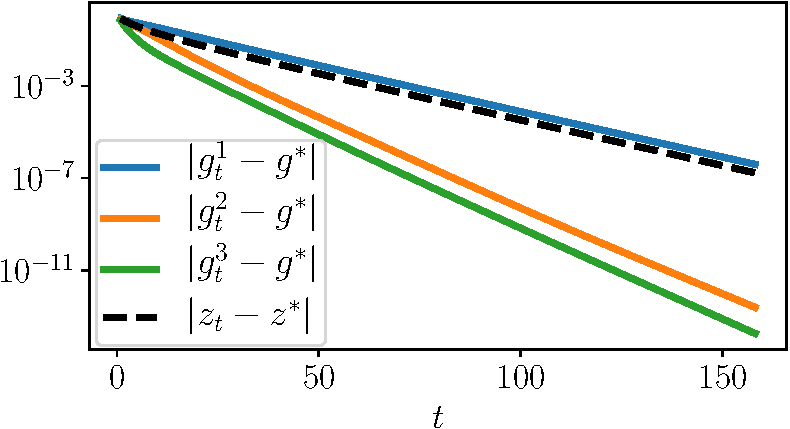
\includegraphics[width=.8\textwidth]{logreg_reg.pdf}\\
        }
    }


\end{document}
